\subsection{序群中的上确界与下确界}

回忆（集合论，III，第141页），若子集 \(F\) （属于有序集 \(E\) ）的上界集合（也就是说，由这样的 \(z \in E\) 组成的集合： \(x \leqslant z\) 对所有 \(x \in F\) 成立）有一个最小元素 \(a\) ，则这个元素（届时是唯一的）称为 \(F\) 的上确界。若 \(F\) 是某个元素族 \((x_{i})_{i \in I}\) （其元素属于 \(E\) ）中元素的集合，则其上确界（若存在）记为 \(\sup_{i \in I} x_i\) （或记为 \(\sup_{i} x_i\) ，或简记为 \(\sup(x_i)\) ）；如果它是一个

有限族 \((x_{\iota})\) \((1 \leqslant \iota \leqslant n)\) ，则该上确界也记为 sup \((x_{1}, \ldots, x_{n})\) 。下确界的定义类似，记为 inf。运算 sup 和 inf 满足结合律和交换律。

回顾（集合论，同上引）若 F 是有序集 E 的一个子集，且 \((x_{t})\) 是 F 中元素的一个族，则 \(\sup(x_{t})\) 在 E 中的存在性（可记为 \(\sup_{E}(x_{t})\) ）并不蕴含 \(x_{t}\) 在 F 中的上确界的存在性（当它存在时可记为 \(\sup_{F}(x_{t})\) ）；若两者都存在，我们只知道 \(\sup_{E}(x_{t}) \leqslant \sup_{F}(x_{t})\) ；然而若 \(\sup_{E}(x_{t})\) 存在且属于 F，则 \(\sup_{F}(x_{t})\) 存在且等于 \(\sup_{E}(x_{t})\) 。例如，在多项式环 A = K{[}X, Y{]} （K 为域）中，主理想 AX 和 AY 在 A 的理想的有序集（按包含关系 ⊂）中具有上确界 AX + AY，但在 A 的所有主理想的集合中具有上确界 A。

（DIV）一个元素 \(d\) （属于 \(\mathbf{K}^*\) ）称为元素族 \((x_{\iota})\) （其元素属于 \(\mathbf{K}^*\) ）的最大公因子，简称 gcd，如果主分式理想 \((d)\) 是 \(\mathcal{P}^*\) 中（在关系 \(\subset\) 下）理想族 \(((x_{\iota}))\) 的上确界，或者换句话说，如果关系 \(z \mid d\) （ \(z \in \mathbf{K}^*\) ）等价于“ \(\ll z \mid x_{\iota}\) 对所有 \(\iota\) ”。同样地，我们将说 \(m \in \mathbf{K}^*\) 是族 \((x_{\iota})\) 的最小公倍元或 lcm，如果 \((m)\) 是 \(\mathcal{P}^*\) 中理想族 \(((x_{\iota}))\) 的下确界，即 \(m \mid z\) 等价于“ \(\ll x_{\iota} \mid z\) 对所有 \(\iota\) ”。这等同于说 \((m) = \bigcap_{\iota} (x_{\iota})\) ；事实上，条件 \(x_{\iota} \mid z\) （对所有 \(\iota\) ）等价于 \(z \in Ax_{\iota}\) （对所有
\(\iota\) ），即 \(z \in \cap (x_{\iota})\) ，而条件 \(m \mid z\) 等价于 \(z \in (m)\) \(^{1}\) 。

\pandocbounded{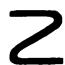
\includegraphics[keepaspectratio]{images/part002_2ca33fff.jpg}}

注意，若主分式理想 \((d)\) 满足 \((d) = \sum_{i} (x_i)\) ，则 \(d\) 是族 \((x_{\iota})\) 的一个最大公因子；但反过来， \((x_{\iota})\) 的最大公因子不一定满足上述条件（参见第六章，第33页，习题24）。

最大公因子和最小公倍元若存在，则在 \(K^{*}\) 的单位组成的子群 U 的模下是良定义的，也就是说，给定族的两个最大公因子（或两个最小公倍元）是相伴元；按语言的滥用，我们常把 \(\gcd(x_{t})\) 与 \(\operatorname{lcm}(x_{t})\) 写作族 \((x_{t})\) 的任意一个最大公因子或最小公倍元，只要这样的元素存在。

（DIV）按语言的滥用，我们有时把最大公因子的概念推广到 K 的元素的族 \((x_{i})\) ，其中某些元素可以是零；这个最大公因子仍定义为这样的元素 d：关系 \(z \mid d\) 等价于“ \(z \mid x_{i}\) 对所有 \(i\) ”；显然，若所有 \(x_{i}\) 均为零，则 d 为零；否则 d 是非零 \(x_{i}\) 的最大公因子。类似地，若一族元素中有一些为零，则其最小公倍元为 0。

在序群 G 中，序在平移下的不变性（VI，第 2 页，命题 2）的一个直接推论是

\[
\sup \left(z + x _ {i}\right) = z + \sup \left(x _ {i}\right)\tag{1}
\]

其含义是，只要一边有定义，则另一边也有定义且两者相等。类似地，由映射 \(x \mapsto -x\) 将 G 的序变为相反序（VI，第 3 页，推论）这一事实可得

\[
\inf (- x _ {i}) = - (\sup (x _ {i})),\tag{2}
\]

此关系与前一个关系作相同理解。

命题6. --- 设 \((x_{\alpha})_{\alpha \in A}, (y_{\beta})_{\beta \in B}\) 是序群G中元素的两个族，每个族都有上确界。则族 \((x_{\alpha} + y_{\beta})_{(\alpha, \beta) \in A \times B}\) 具有上确界，并且 \(\sup_{(\alpha, \beta) \in A \times B} (x_{\alpha} + y_{\beta}) = \sup_{\alpha \in A} x_{\alpha} + \sup_{\beta \in B} y_{\beta}\) 。

确实，由 \(x_{\alpha} + y_{\beta} \leqslant z\) （对所有 \(\alpha\) 与 \(\beta\) ）可推出 \(\sup (x_{\alpha}) + y_{\beta} \leqslant z\) （对所有 \(\beta\) ），从而 \(\sup (x_{\alpha}) + \sup (y_{\beta}) \leqslant z\) 。

